\documentclass{article}
\usepackage{fullpage}
\usepackage[utf8]{inputenc}
\usepackage{graphicx}
\usepackage[ngerman]{babel}
\usepackage{hyperref}
\usepackage{tabularx}
\usepackage{attachfile}
\usepackage{pdfpages}
\usepackage{siunitx}
\usepackage{caption} \captionsetup[table]{skip=10pt}
\usepackage{graphicx}
\usepackage{subfig}
\usepackage{float}
\usepackage{gensymb}

\title{Ausarbeitung zu Viskosität (VIS)}
\author{Anfängerpraktikum Teil 1 \\Technische Universität München\\\\Leon Heiß, Paul Hildebrandt \\
Kurs 5, Gruppe 7, Team 19}
\date{12. Juli 2022}
\renewcommand*\contentsname{Inhaltsverzeichnis}

\begin{document}

\maketitle

\large
\begin{center}
\textbf{Abstract}\\
\normalsize
\medskip
Das Ziel dieses Versuchs ist es, die Viskosität verschiedener Flüssigkeiten mithilfe eines Kugelfallviskosimeters und Kapillarviskosimeters zu bestimmen.

\end{center}
\normalsize

\tableofcontents
\section{Grundlagen}
\subsection{Viskosität}
Die $\textit{Viskosität}$ eines Fluids beschreibt wie zähflüssig dieses ist. Genauer ist die $\textit{dynamische Viskosität}$ $\eta$
eine materialabhängige Proportionalitätskonstante der inneren Reibung eines Fluids. Die Viskosität ist temperaturabhängig, in den meisten Fällen steigt sie bei Gasen und sinkt bei Flüssigkeiten bei zunehmender Temperatur.
Mithilfe der Dichte $\rho$ des Fluids lässt sich dessen $\textit{kinematische Viskosität}$ berechnen:
\begin{equation}
    \nu = \frac{\eta}{\rho}.
\end{equation}
In einer $\textit{Newtonschen Flüssigkeit}$ ist die Viskosität $\eta$ unabhängig von deren Geschwindigkeit, das Geschwindigkeitsprofil ist also linear. Ist das nicht der Fall, heißt die Flüssigkeit $\textit{nicht-Newtonsch}$.
\subsection{Laminare und turbulente Strömungen}
Bei $\textit{laminarer Strömung}$ gleiten Flüssigkeitsschichten gleichmäßig aneinander vorbei, dies ist meist bei niedrigen Flussgeschwindigkeiten und an stromlinienförmigen Objekten der Fall. Für größeren Flussgeschwindigkeiten oder nicht-stromlinienförmige Körper treten Verwirbelungen auf und die Stromlinie reißt ab. Dies nennt man dann $\textit{turbulente Strömung}$. Der Unterschied zwischen den Strömungen ist in den
Abbildungen 1a und 1b veranschaulicht.
Mithilfe der $\textit{Reynoldszahl}$ $ R_e$ kann man berechnen, welche Strömung in einem System zu erwarten ist:
\begin{equation}
    R_e = \frac{L \cdot \rho \cdot \nu_{mittel}}{\eta},
\end{equation}
wobei $\nu_{mittel}$ die mittlere Geschwindigkeit und $L$ die $\textit{charakteristische Länge}$ des Systems ist. Für letztere gilt bei einer Strömung in einem Rohr mit Innendurchmesser $d$, dass $L = d$. Für ein Rohr hat man für $R_e < 1160$ laminare Strömung und für $2300 < R_e$ turbulente Strömung. Im Bereich dazwischen können Verwirblungen durch Einlaufstörungen auftreten.
\begin{figure}[H]
    \centering
    \subfloat[\centering Laminare Strömung]{{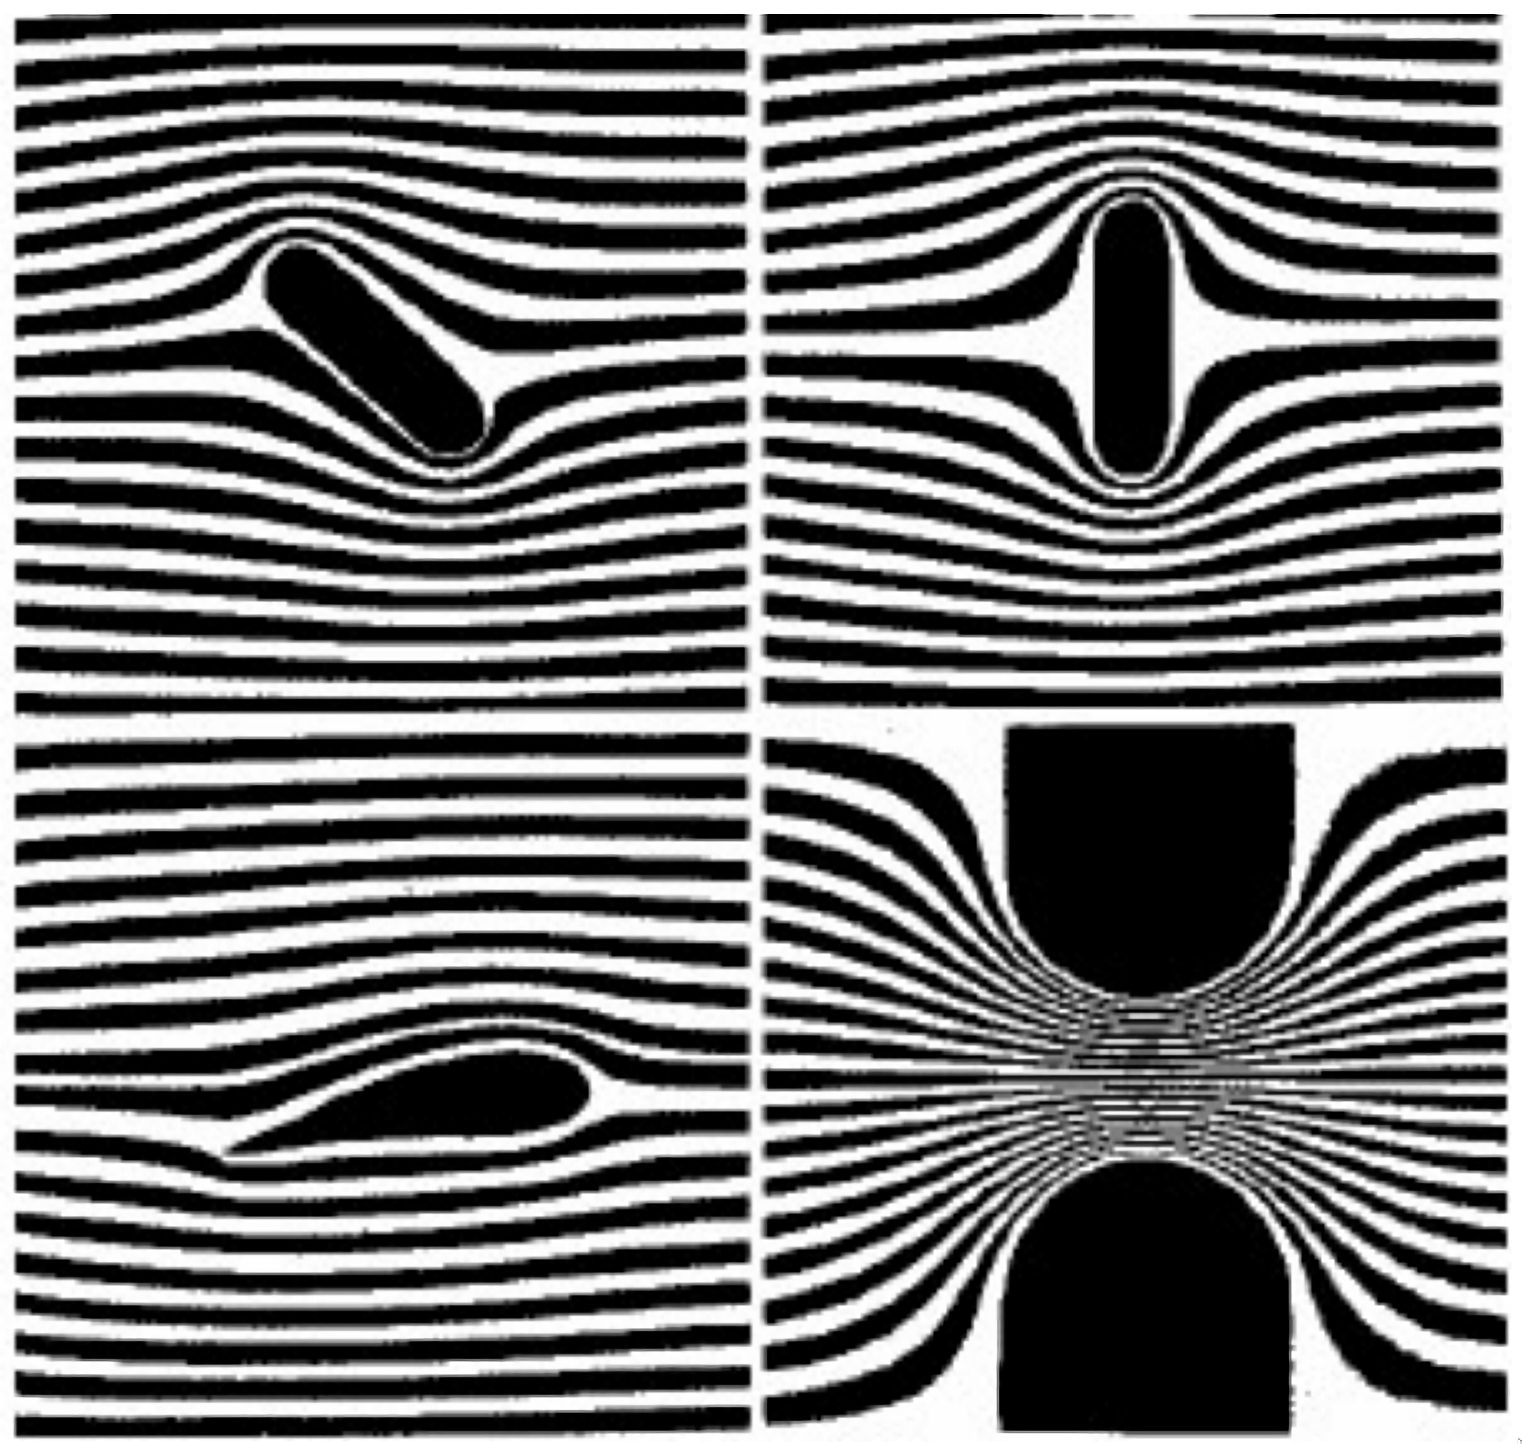
\includegraphics[width=5cm]{laminar.png} }}%
    \qquad
    \subfloat[\centering Turbulente Strömung]{{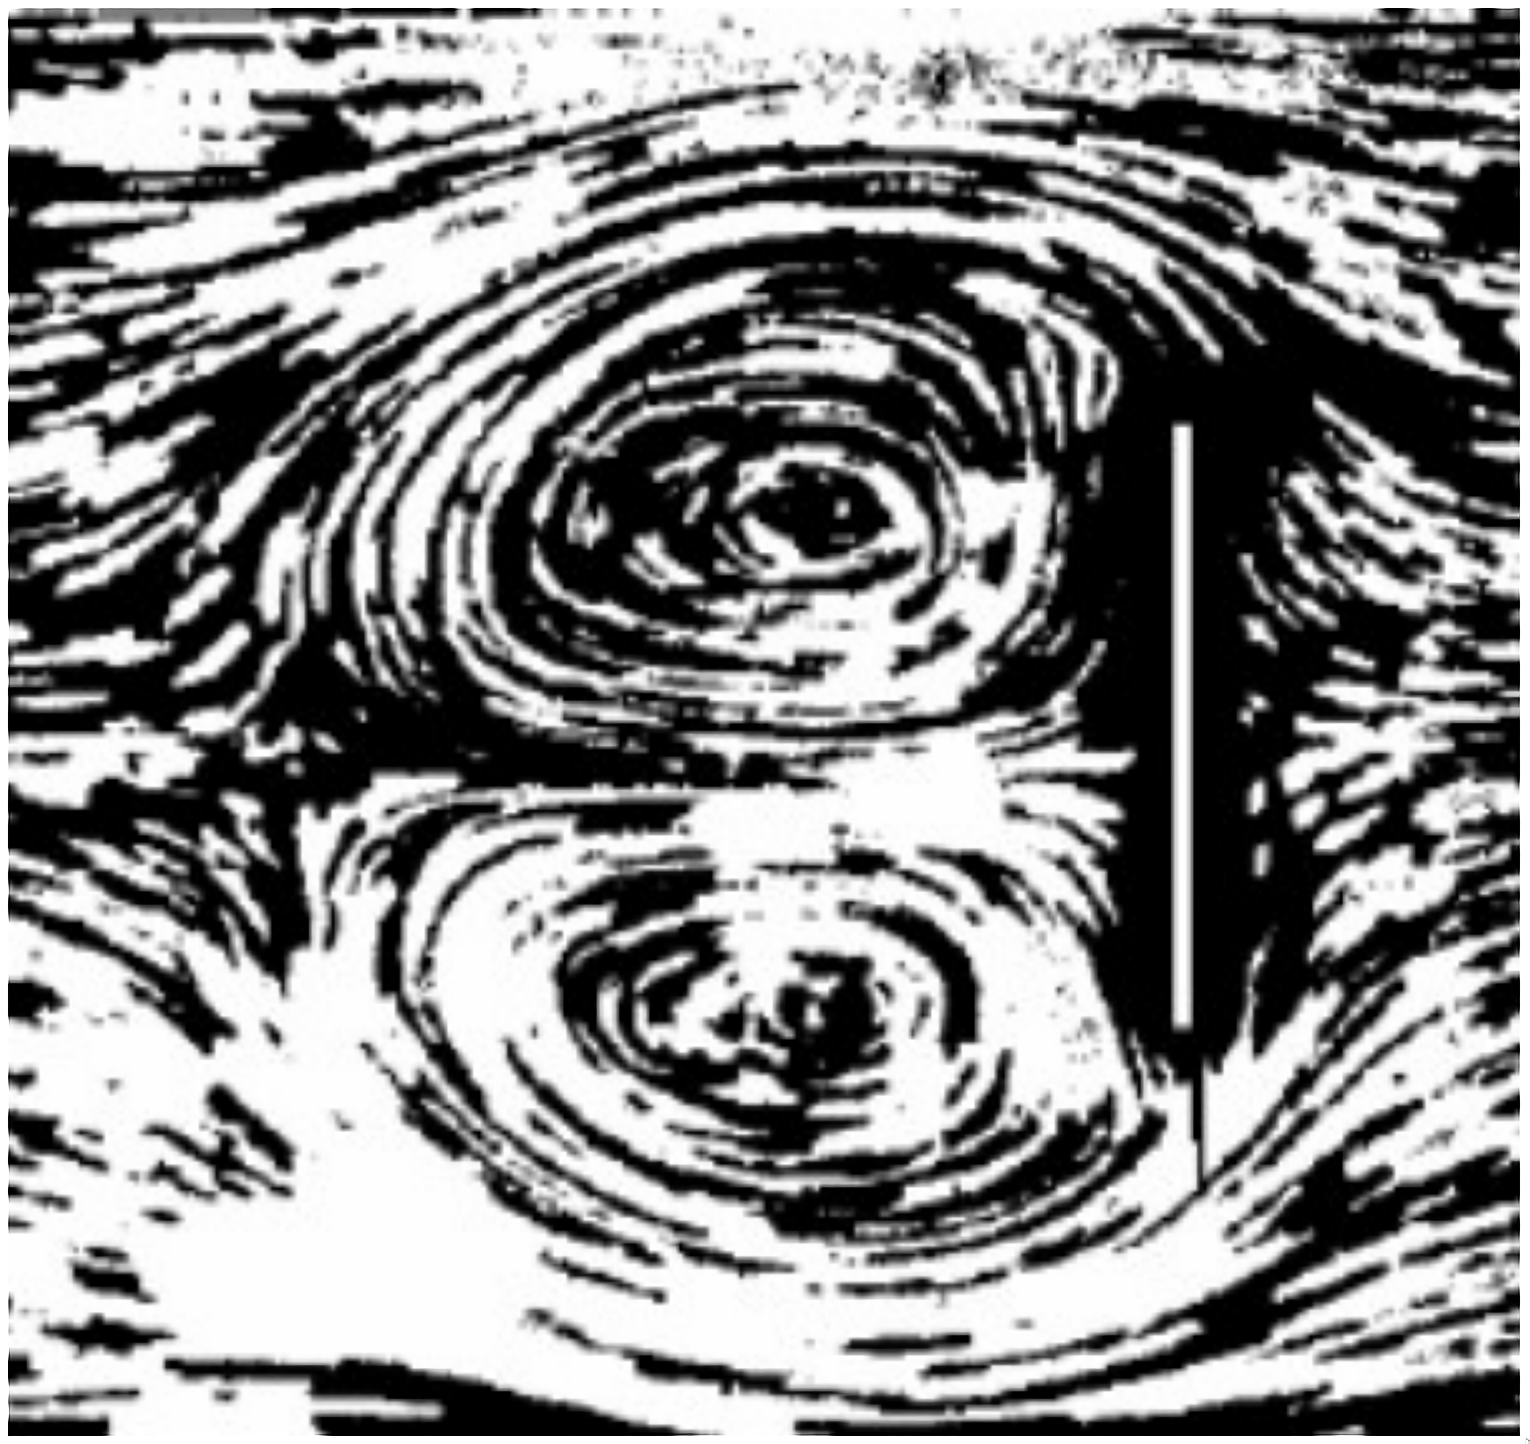
\includegraphics[width=5cm]{turb.png} }}%
    \caption{Vergleich der beiden Strömungsarten \cite{1}}
    \label{fig:example}%
\end{figure}
\subsection{Hagen-Poiseuillsche Gesetz}
Die Stromstärke $i$ einer Flüssigkeitsströmung gibt an, wie viel Volumen einen Querschnitt $A$ pro Zeit passiert. Für ein Rohr mit Radius $r$, Länge $l$ und Druckdifferenz $\Delta p = p_1 - p_2$ gilt mit Hagen-Poiseuillsche Gesetz \cite{1}:
\begin{equation}
    i = \frac{\pi \cdot r^4 \cdot \Delta p}{8 \cdot \eta \cdot l} = A \cdot \nu_{mittel}.
\end{equation}
Das Gesetz ist jedoch lediglich eine Näherung, welche nur gilt, wenn keine äußeren und Trägheitskräfte wirken, die Strömung laminar, der Rohrradius konstant, das Medium inkompressibel und die Randgeschwindigkeit $\nu = 0$ ist.
\subsection{Bernoulli Gleichung}
Zur Berechnung der Druckdifferenz $\Delta p$ kann die Bernoulli Gleichung verwendet werden:
\begin{equation}
    p + \rho g h +\frac{1}{2} \nu^2 = \textrm{konst.}
\end{equation}
Betrachtet man $\Delta p = p_1 - p_2$ für ein vertikal stehendes Rohr ergibt sich
\begin{equation}
    \Delta p = \rho g \Delta h,
\end{equation}
dabei steht $\Delta h$ für die Höhendifferenz des Rohres.
\subsection{Strömungswiderstand}
Der $\textit{Strömungswiderstand}$ $W$ ist ein Maß dafür, wie stark die Strömung durch Gegenkräfte gebremst wird. Es gilt
\begin{equation}
    W = \frac{8 \cdot \eta \cdot l}{\pi r^4}.
\end{equation}
Damit lässt sich das Hagen-Poiseuille umformen zu
\begin{equation}
    \Delta p = W \cdot i.
\end{equation}
Für Newtonsche Flüssigkeiten gilt, dass $W$ die Steigung im Druckdifferenz-Stromstärke-Diagramm ist.
\subsection{Stokessche Gesetz}
Die Viskosität spielt eine zentrale Rolle bei Sinkbewegungen von Körpern in Flüssigkeiten. Betrachtet
man beispielsweise eine Kugel vom Radius $r$, die in einem unendlich ausgedehnten, zähen Medium mit
konstanter Geschwindigkeit $\nu$ nach unten sinkt, lassen sich die dabei wirkenden Kräfte folgendermaßen
grafisch darstellen:
\begin{figure}[H]
\centering
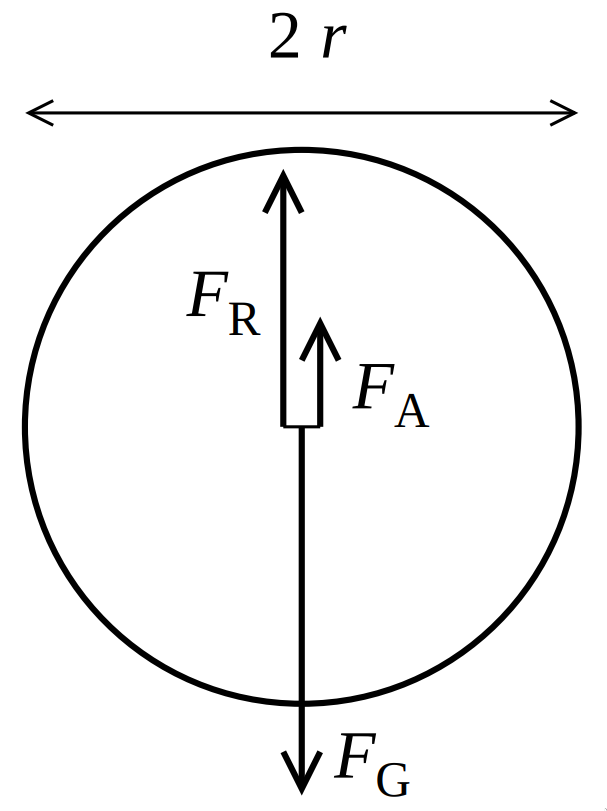
\includegraphics[width=110pt]{stokes.png}
\caption{Fallende Kugel im zähen Medium \cite{1}}
\label{fig:length_eight_mouse}
\end{figure}
\noindent
Die in Abbildung 2 eingezeichnete Gewichtskraft $F_G = m \cdot g$ zeigt in Richtung der Fallbewegung. Dazu
entgegengerichtet wirken die Auftriebskraft $F_A = V_{Kugel} \cdot \rho_{Fl} \cdot g$ und die Stokessche Reibungskraft $F_R = 6 \pi \cdot \eta \cdot r \cdot \nu$ \cite{1}, wobei diese Gleichung nur bei laminarer Strömung gültig ist. Die Reynoldszahl muss für diese Art der Strömung hier im Gegensatz zur Rohrströmung Werte kleiner als eins annehmen. Stellt man das Kräftegleichgewicht $\vert F_G \vert = \vert F_A \vert + \vert F_R \vert $ auf und formt nach $\eta$ um, erhält man
\begin{equation}
    \eta = \frac{2 \cdot r^2 \cdot g}{9 \cdot \nu} \cdot (\rho_{Kugel} - \rho_{Fl})
\end{equation}
als Ausdruck für die Viskosität der Flüssigkeit. Will man die Viskosität mit dieser Methode nicht für einen unendlich ausgedehnten Raum, sondern für ein Rohr mit Radius $R$ berechnen, muss man bei Gleichung 8 noch einen Korrekturfaktor einfügen:
\begin{equation}
    \eta = \frac{2 \cdot r^2 \cdot g}{9 \cdot \nu \cdot (1+2,4 \cdot \frac{r}{R})} \cdot (\rho_{Kugel} - \rho_{Fl}).
\end{equation}
\section{Kugelfallviskosimeter}
\subsection{Versuchsaufbau}
\begin{figure}[H]
\centering
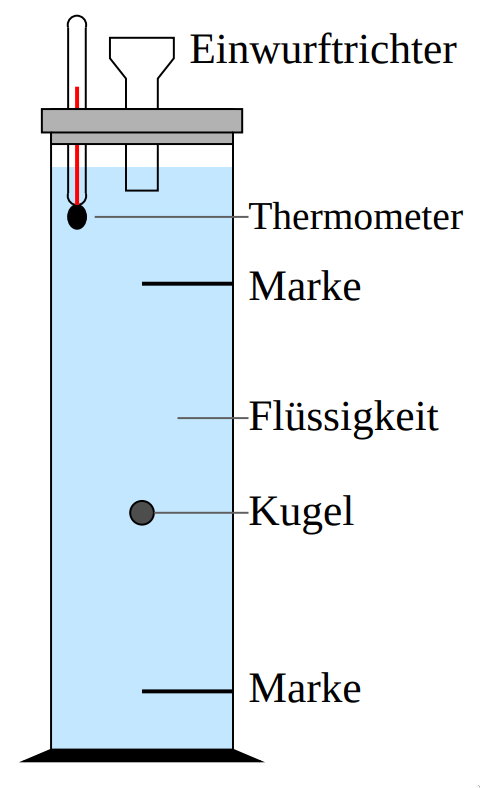
\includegraphics[width=140pt]{kugelfall.png}
\caption{Versuchsaufbau Kugelfallviskosimeter \cite{1}}
\label{fig:length_eight_mouse}
\end{figure}
Das Kugelfallviskosimeter (Abbildung 1) ist eine besondere Bauform eines Viskosimeters und dient der präzisen Messung der Viskosität durchsichtiger newtonscher Flüssigkeiten. Es besteht aus einem zylindrischen Behälter, welcher mit einem Glyzerin-Wasser Gemisch gefüllt ist. Für den Versuch werden zunächst die Massen und Durchmesser zehn kleiner, gleich großer Kugeln bestimmt. Diese lässt man anschließend nacheinander durch den Einwurftrichter im Glyzerin-Wasser Gemisch innerhalb des Viskosimeters nach unten sinken. Währenddessen stoppt man für jede der Kugeln die Zeit, die diese benötigen, um die in der Abbildung markierte Strecke innerhalb des Fallrohres zurückzulegen.
Nun wird noch die Flüssigkeitsdichte mithilfe eines Aräometer bestimmt, sowie der Innenrohrradius des Kugelfallviskosimeters ausgemessen.
\newpage
\subsection{Auswertung}
Mithilfe der Gleichungen 8 und 9 ergibt sich die unkorrigierte Viskosität des Glyzerin-Wasser Gemischs zu $\eta = 169 \pm 69$ mPa s und die korrigierte Variante zu $\eta_{korr} = 89 \pm 61$ mPa s. Eine detallierte Berechnung der involvierten Unsicherheiten ist im nächsten Abschnitt zu finden.
Vergleicht man die ermittelten Werte für die korrigierte bzw. unkorrigierte Viskosität mit Abbildung 4, entsprechen die Daten einer Konzentration von ca. $87\%$ des Glyzerin-Wasser Gemischs bei einer Temperatur von $20\degree$C. Da unsere Messungen jedoch bei $23 \degree$C gemacht wurde, ist dies nicht unbedingt aussagekräftig über die Genauigkeit.
\begin{figure}[H]
\centering
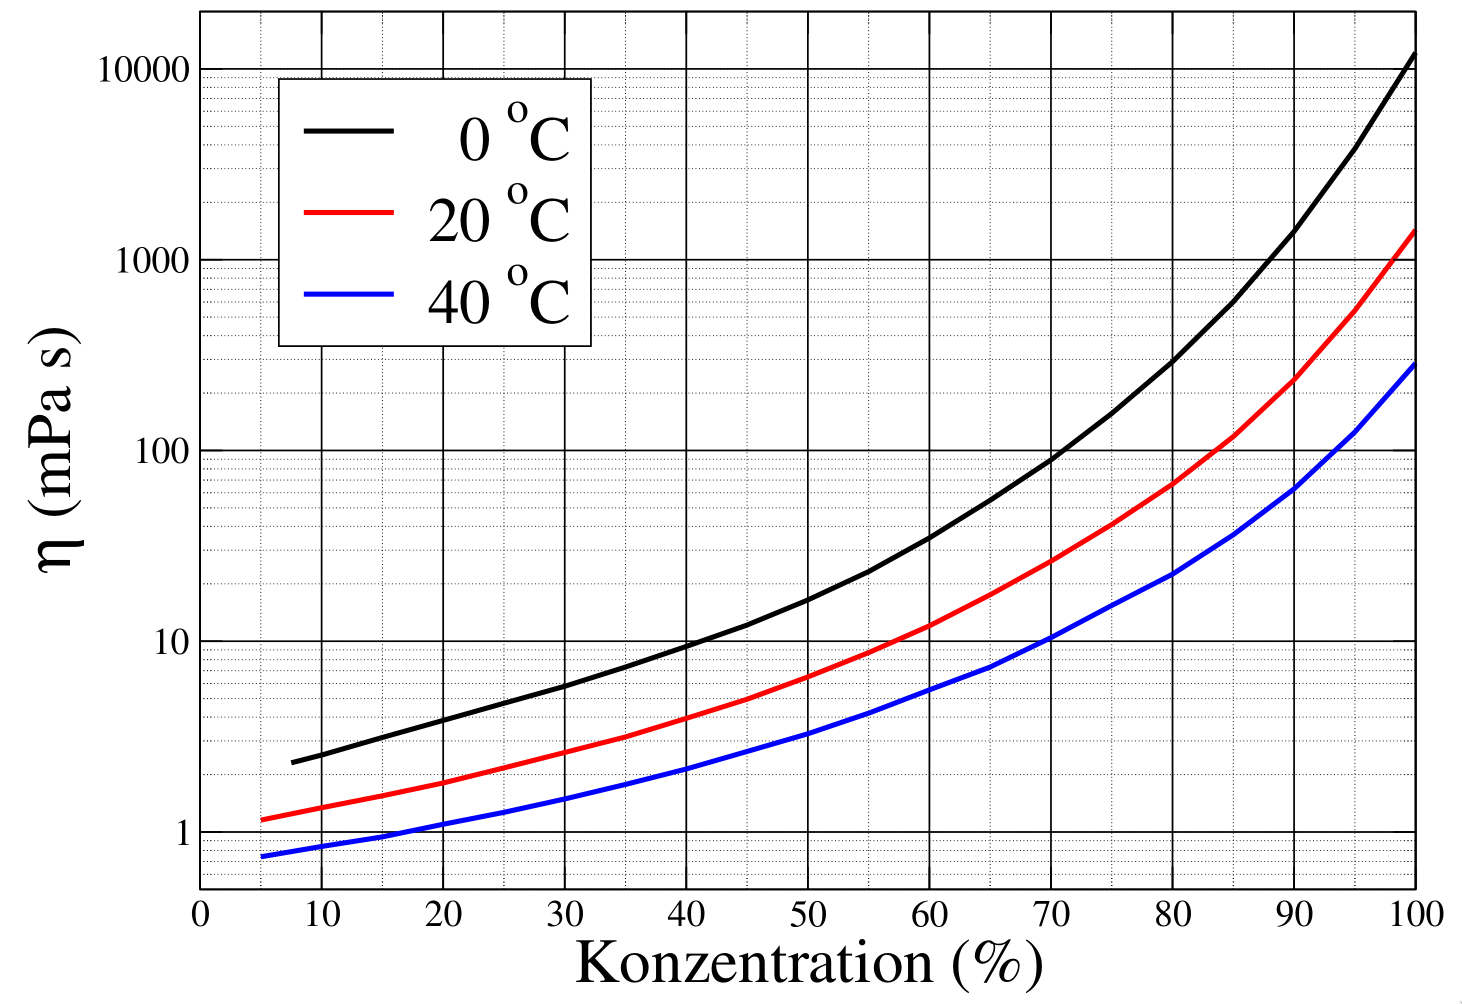
\includegraphics[width=300pt]{vis-konzentration.png}
\caption{Viskosität in Abhängigkeit von der Konzentration des Glyzerin-Wasser Gemischs \cite{1}}
\label{fig:length_eight_mouse}
\end{figure}
\noindent
Nun können wir mithilfe von Gleichung 2 die Reynoldszahl $R_e = 410 \pm 186$ ermitteln, wobei der unkorrigierte Wert für die Viskosität verwendet wurde. Da die Reynoldszahl deutlich unter 1160 liegt, handelt es sich hierbei um eine laminare Strömung. Die Unsicherheit für die Reynoldszahl wurde hier ebenfalls mithilfe der Gaußschen Fehlerfortpflanzung bestimmt.
\subsection{Fehlerrechnung} 
Gleichung 8 kann mit $v = \frac{h}{t}$ und $\rho_K = \frac{m}{\frac{4}{3} \pi r^3}$ zu
\begin{equation}
    \eta = \frac{2gr^2 \cdot t}{9h} \cdot \bigg(\frac{3m}{4\pi r^3} - \rho \bigg)
\end{equation}
umgeschrieben werden. Dieser Ausdruck hängt insgesamt von fünf unterschiedlichen Parametern ab, deren
Unsicherheiten im Folgenden einzeln diskutiert werden sollen. Um die Gaußsche Fehlerfortpflanzung mit
möglichst kleinem Aufwand berechnen zu können, bringt man sie auf folgende Form:
\begin{equation}
    u(\eta) = \eta \cdot \sqrt{\bigg(A_{t}\cdot \frac{u(t)}{t}\bigg)^2 + \bigg(A_{h}\cdot \frac{u(h)}{h}\bigg)^2 + \bigg(A_{m}\cdot \frac{u(m)}{m}\bigg)^2 + \bigg(A_{\rho}\cdot \frac{u(\rho)}{\rho}\bigg)^2 + \bigg(A_{r}\cdot \frac{u(r)}{r}\bigg)^2}.
\end{equation}
$A_i$ sind die Vorfaktoren, die entstehen, wenn man Gleichung 11 partiell nach $x_i$ ableitet und anschließend
auf die Form $A_i \cdot \frac{\eta}{x_i}$ bringt.
\paragraph{Zeit t}
Die Unsicherheit in der Zeitmessung $u(t) = \sqrt{u_A(t)^2+ u_B(t)^2}$ setzt sich zusammen aus der Typ-A Unsicherheit $ u_A(t)= 0,057$ s der einzelnen Zeitmessungen, sowie einer zweifachen durchschnittlichen menschlichen Reaktionszeit von $u_B(t) = 0,5$ s. Leitet man Gleichung 8 partiell nach $t$ ab, ergibt sich $\frac{\delta \eta}{\delta t} = \frac{\eta}{t}$ mit dem Vorfaktor $A_t = 1$.
\paragraph{Fallstrecke h}
Die Fallstrecke $h$, welche mit einem Meterstab bestimmt wurde, unterliegt zwei Unsicherheiten. Zunächst wäre da die Ungenauigkeit des Meterstabs $a+b \cdot L$, mit $a = 0,6$ mm, $b = 0,4$ mm/m und $L$ der auf den nächsten vollen Meter aufgerundeten, gemessenen Länge. Diese kommt zu $0,75$ mm. Des Weiteren muss die Ableseungenauigkeit berücksichtig werden, welche wir mit $0,1$ cm abschätzten. Insgesamt kommt man auf eine Unsicherheit der Fallstrecke $h$ von $u(h)=1,25$ mm. Es ergibt sich $ \frac{\delta \eta}{\delta h} = \frac{\eta}{h}$ mit dem Vorfaktor $A_h = -1$. 
\paragraph{Masse m}
Die Unsicherheit in der Messung der Masse $u(m) = \sqrt{u_{B1}(m)^2 + u_{B2}(m)^2}$ g setzt sich zusammen aus der Linearitäts- und Skalierungsunsicherheit der Waage zu $u_{B1}(m)= 0.0005$ g, sowie der Reproduzierbarkeit $u_{B2}(m)= 0.0002$ g. Insgesamt kommt man so auf eine Unsicherheit $u(m)=0,00054$ g. Es ergibt sich $\frac{\delta  \eta}{\delta m} = \frac{\rho_K}{\rho_K - \rho_{Fl}} \cdot \frac{\eta}{m}$ mit dem Vorfaktor $A_m = \frac{\rho_K}{\rho_k - \rho_{Fl}}$. 
\paragraph{Dichte der Flüssigkeit $\rho_{Fl}$}
Das Messen mit dem Aräometer unterliegt zwei Unsicherheiten. Eine Typ-B Unsicherheit von $0,0001 \frac{\textrm{g}}{\textrm{cm}^3}$ \cite{6} und eine geschätzte Ableseungenauigkeit von $0,005 \frac{\textrm{g}}{\textrm{cm}^3}$. Es ergibt sich $\frac{\delta \eta}{\delta \rho_{Fl}} = \frac{\eta}{\rho_{Fl}}$ mit dem Vorfaktor $A_{\rho_{Fl}} = - \frac{\rho_{Fl}}{\rho_K - \rho_{Fl}}$. 
\paragraph{Kugelradius r}
Ähnlich wie bei der Fehlerrechnung zur Fallhöhe bestimmen wir die Messabweichung des Messschiebers zu $u(r)=0,05$ mm.
Die Standardabweichung der gemessenen Kugelradien ergibt sich bei uns zu null, da alle gemessenen Werte miteinander übereinstimmen. Es ergibt sich $\frac{\delta \eta}{\delta r}=\frac{\eta}{r}$ mit Vorfaktor $A_{r} = (2-3 \cdot \frac{\rho_K}{\rho_K - \rho_{Fl}})$.
\paragraph{Viskosität $\eta$}
Setzt man alle $u(x_i)$ und $A_i$ in Gleichung 11 ein, kann man nun die Unsicherheit der unkorrigierten Viskosität bestimmen. Um die Unsicherheit der korrigierten Viskosität zu bekommen, berücksichtigt man die neuen Terme aus Gleichung 9 oder um ein ungefähres Ergebnis für $u(\eta_{korr})$ zu bekommen, multipliziert man $u(\eta)$ mit dem Faktor $\frac{1}{1+2,4 \cdot \frac{r}{R}}$.
\section{Kapillarviskosimeter}
\subsection{Versuchsaufbau}
\begin{figure}[H]
\centering
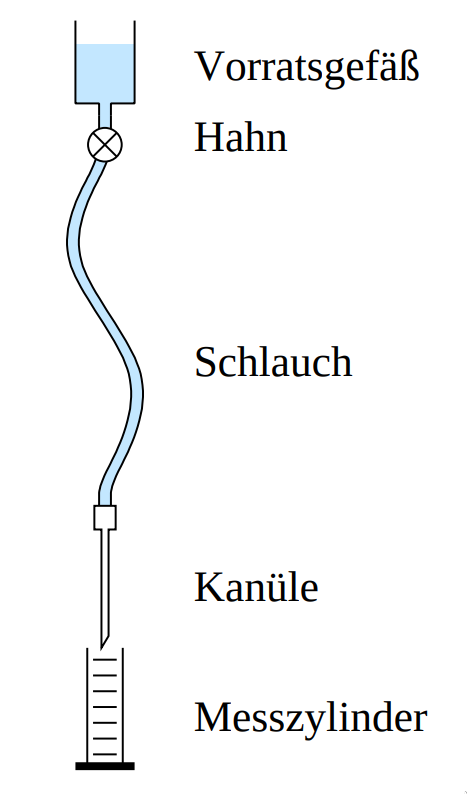
\includegraphics[width=150pt]{kapillar.png}
\caption{Versuchsaufbau Kapillarviskosimeter \cite{1}}
\label{fig:length_eight_mouse}
\end{figure}
Beim Kapillarviskosimeter, zu sehen in Abbildung 5, fließt Wasser aus einem Vorratsbehältnis durch einen Schlauch in eine darunter liegende Kapillare, in diesem Fall eine Injektionskanüle. Mithilfe der Höhe des Behälters relativ zur Kanüle kann der Druck in der Kapillare variiert werden. Die Menge des während einer gemessenen Zeitspanne durch die Kapillare gelaufenen Wassers wir durch das Wiegen des Auffangbehältnisses vor und nach dem Versuch bestimmt.
\subsection{Auswertung}
Im Folgenden soll die Viskosität der Flüssigkeit bestimmt werden. Dazu wird der Druck, wie unter Gleichung 7 angedeutet, gegen die Stromstärke aufgetragen. Der Druck lässt sich aus der Höhe der Leitung durch
\begin{equation}
p(h) = \rho \cdot g \cdot h
\end{equation}
bestimmen. Für die Temperatur von 23$ \degree $C wird eine Dichte von 997,54 $\frac{\textrm{kg}}{\textrm{m}^3}$ verwendet $\cite{8}$. Die Steigung der Ausgleichsgerade (Abbildung 6) entspricht dem Strömungswiderstand. Jeglicher Offset entlang der Druck-Achse hat keinerlei Auswirkungen.
\begin{figure}[H]
\centering
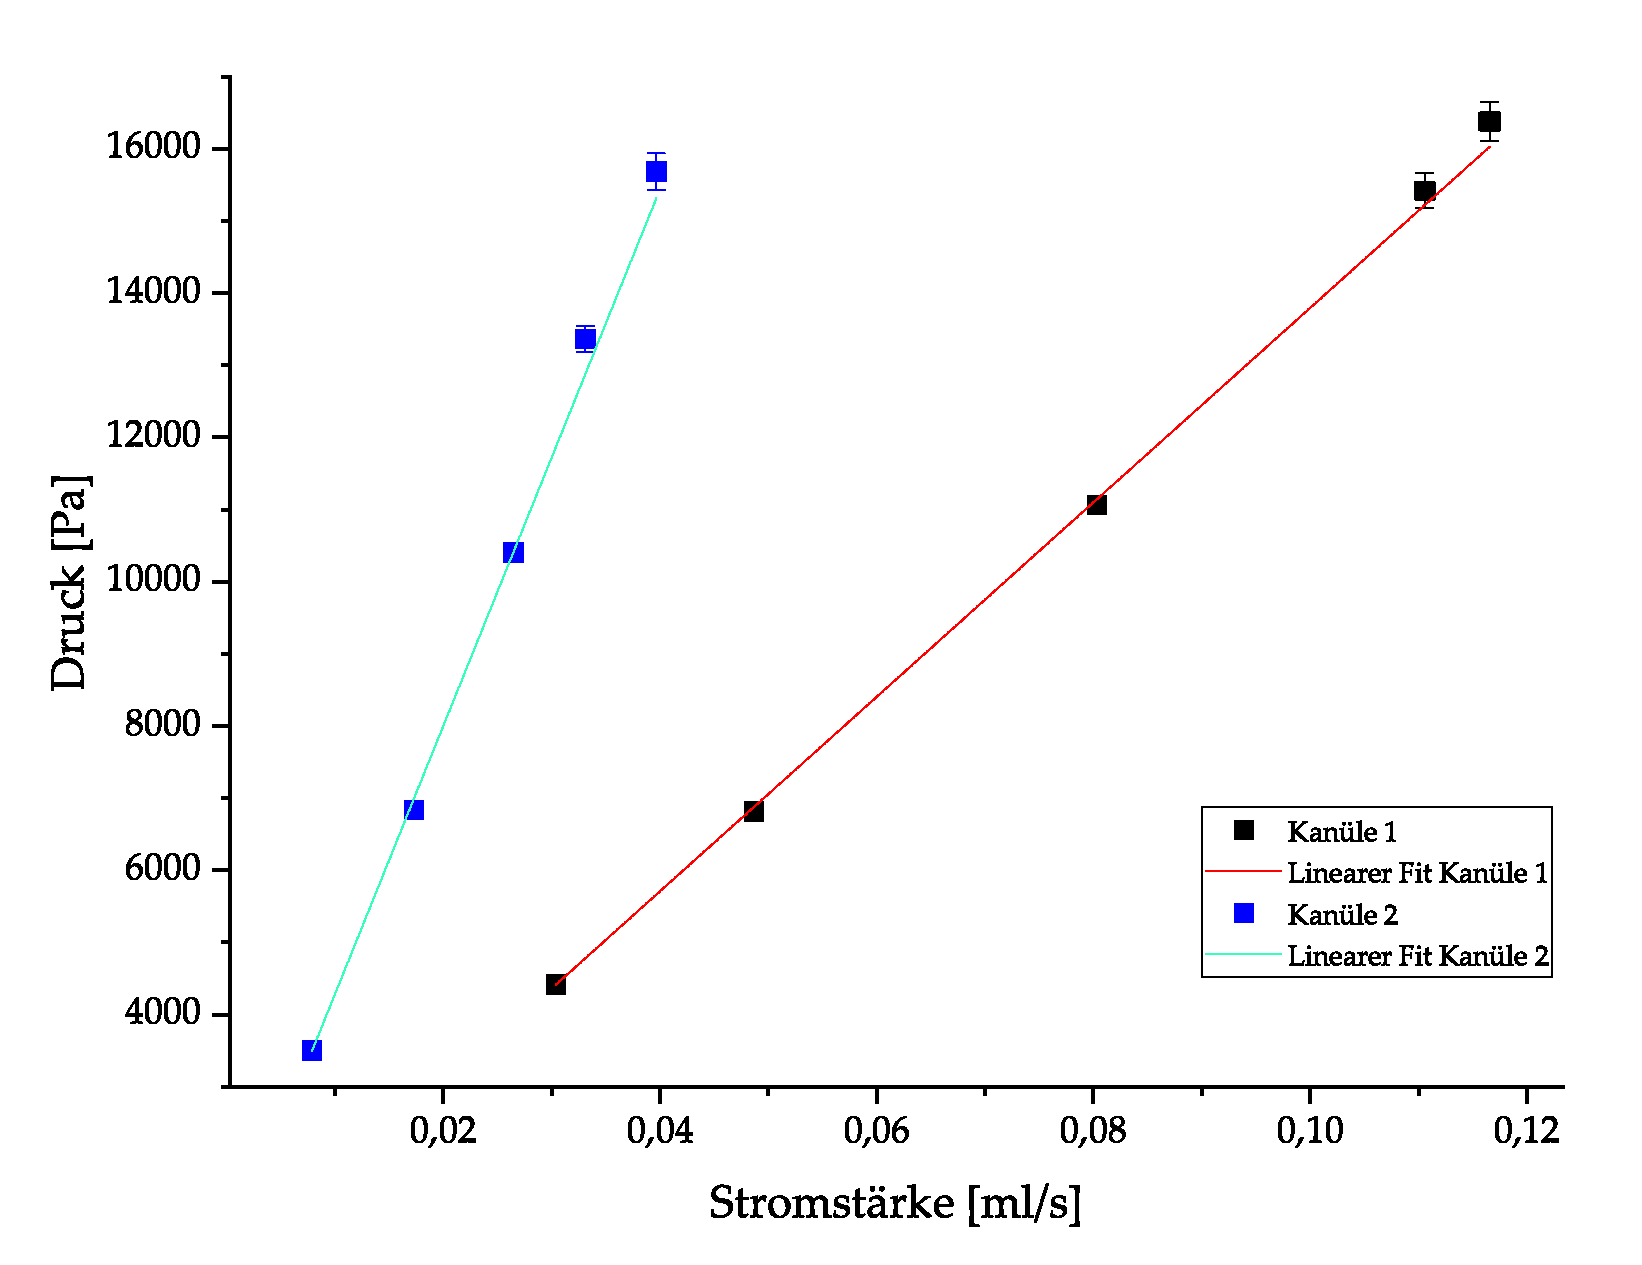
\includegraphics[width=350pt]{DruckStrom.eps}
\caption{Druck bei verschiedenen Stromstärken in beiden Kanülen und zugehörige Ausgleichsgeraden}
\label{fig:length_eight_mouse}
\end{figure}
\noindent
Aus den Werten des Strömungswiderstandes von $134,74\cdot 10^9 \pm 1,81 \cdot 10^9 \   \frac{\textrm{Pa}\cdot \textrm{s}}{\textrm{m}^3}$ für Kanüle 1 und $371,90\cdot 10^9 \pm 8,33\cdot 10^9 \ \frac{\textrm{Pa}\cdot \textrm{s}}{\textrm{m}^3}$ für Kanüle 2 lässt sich mithilfe des Zusammenhangs
\begin{equation}
\eta = \frac{W\cdot\pi\cdot r^4}{8\cdot l}
\end{equation}
ein Wert von $1,030 \pm 0,593 \ \textrm{mPa} \cdot \textrm{s}$ in Kanüle 1 und ein Wert von $0,498 \pm 0,315 \ \textrm{mPa} \cdot \textrm{s}$ für die Viskosität der Flüssigkeit bei $23 \degree$C bestimmen. Die hohe Unsicherheit kommt zu großem Teil dadurch zustande, dass der Radius, der mit einer Unsicherheit von etwa 10$\%$ geschätzt wird, mit der 4. Potenz in die Berechnung einfließt. Kleine Änderungen am Radius können große Änderungen am Endgültigen Wert bewirken. So müsste man den gemessenen Wert von 9,5 Sktl um nur 1,5 Sktl erhöhen, um dem Literaturwert von $0,960 \ \textrm{mPa}\cdot \textrm{s}$ \cite{9} bei 23$ \degree$C zu erhalten. Der Wert für Kanüle 1 liegt nah am Literaturwert.
\subsection{Fehlerrechnung}
Unsicherheiten für Zeit, Höhe und Masse wurden wie in Abschnitt 2.3 erläutert, berechnet. 
\paragraph{Dichte} Für den Literaturwert der Dichte \cite{8} wurde die letzte verwendete Stelle, also $0,001\frac{\textrm{kg}}{\textrm{m}^3}$ als unsicher angenommen.
\paragraph{Länge der Kapillare} Die Kapillare ist an einem Ende schräg angeschnitten. Ein eindeutiges Ende ist also nicht direkt zu bestimmen. Für unsere Auswertung wurde der Mittelpunkt der Schräge für die Längenbestimmung verwendet und die Unsicherheit wie in Abbildung 7 dargestellt, bestimmt.
\begin{figure}[H]
\centering
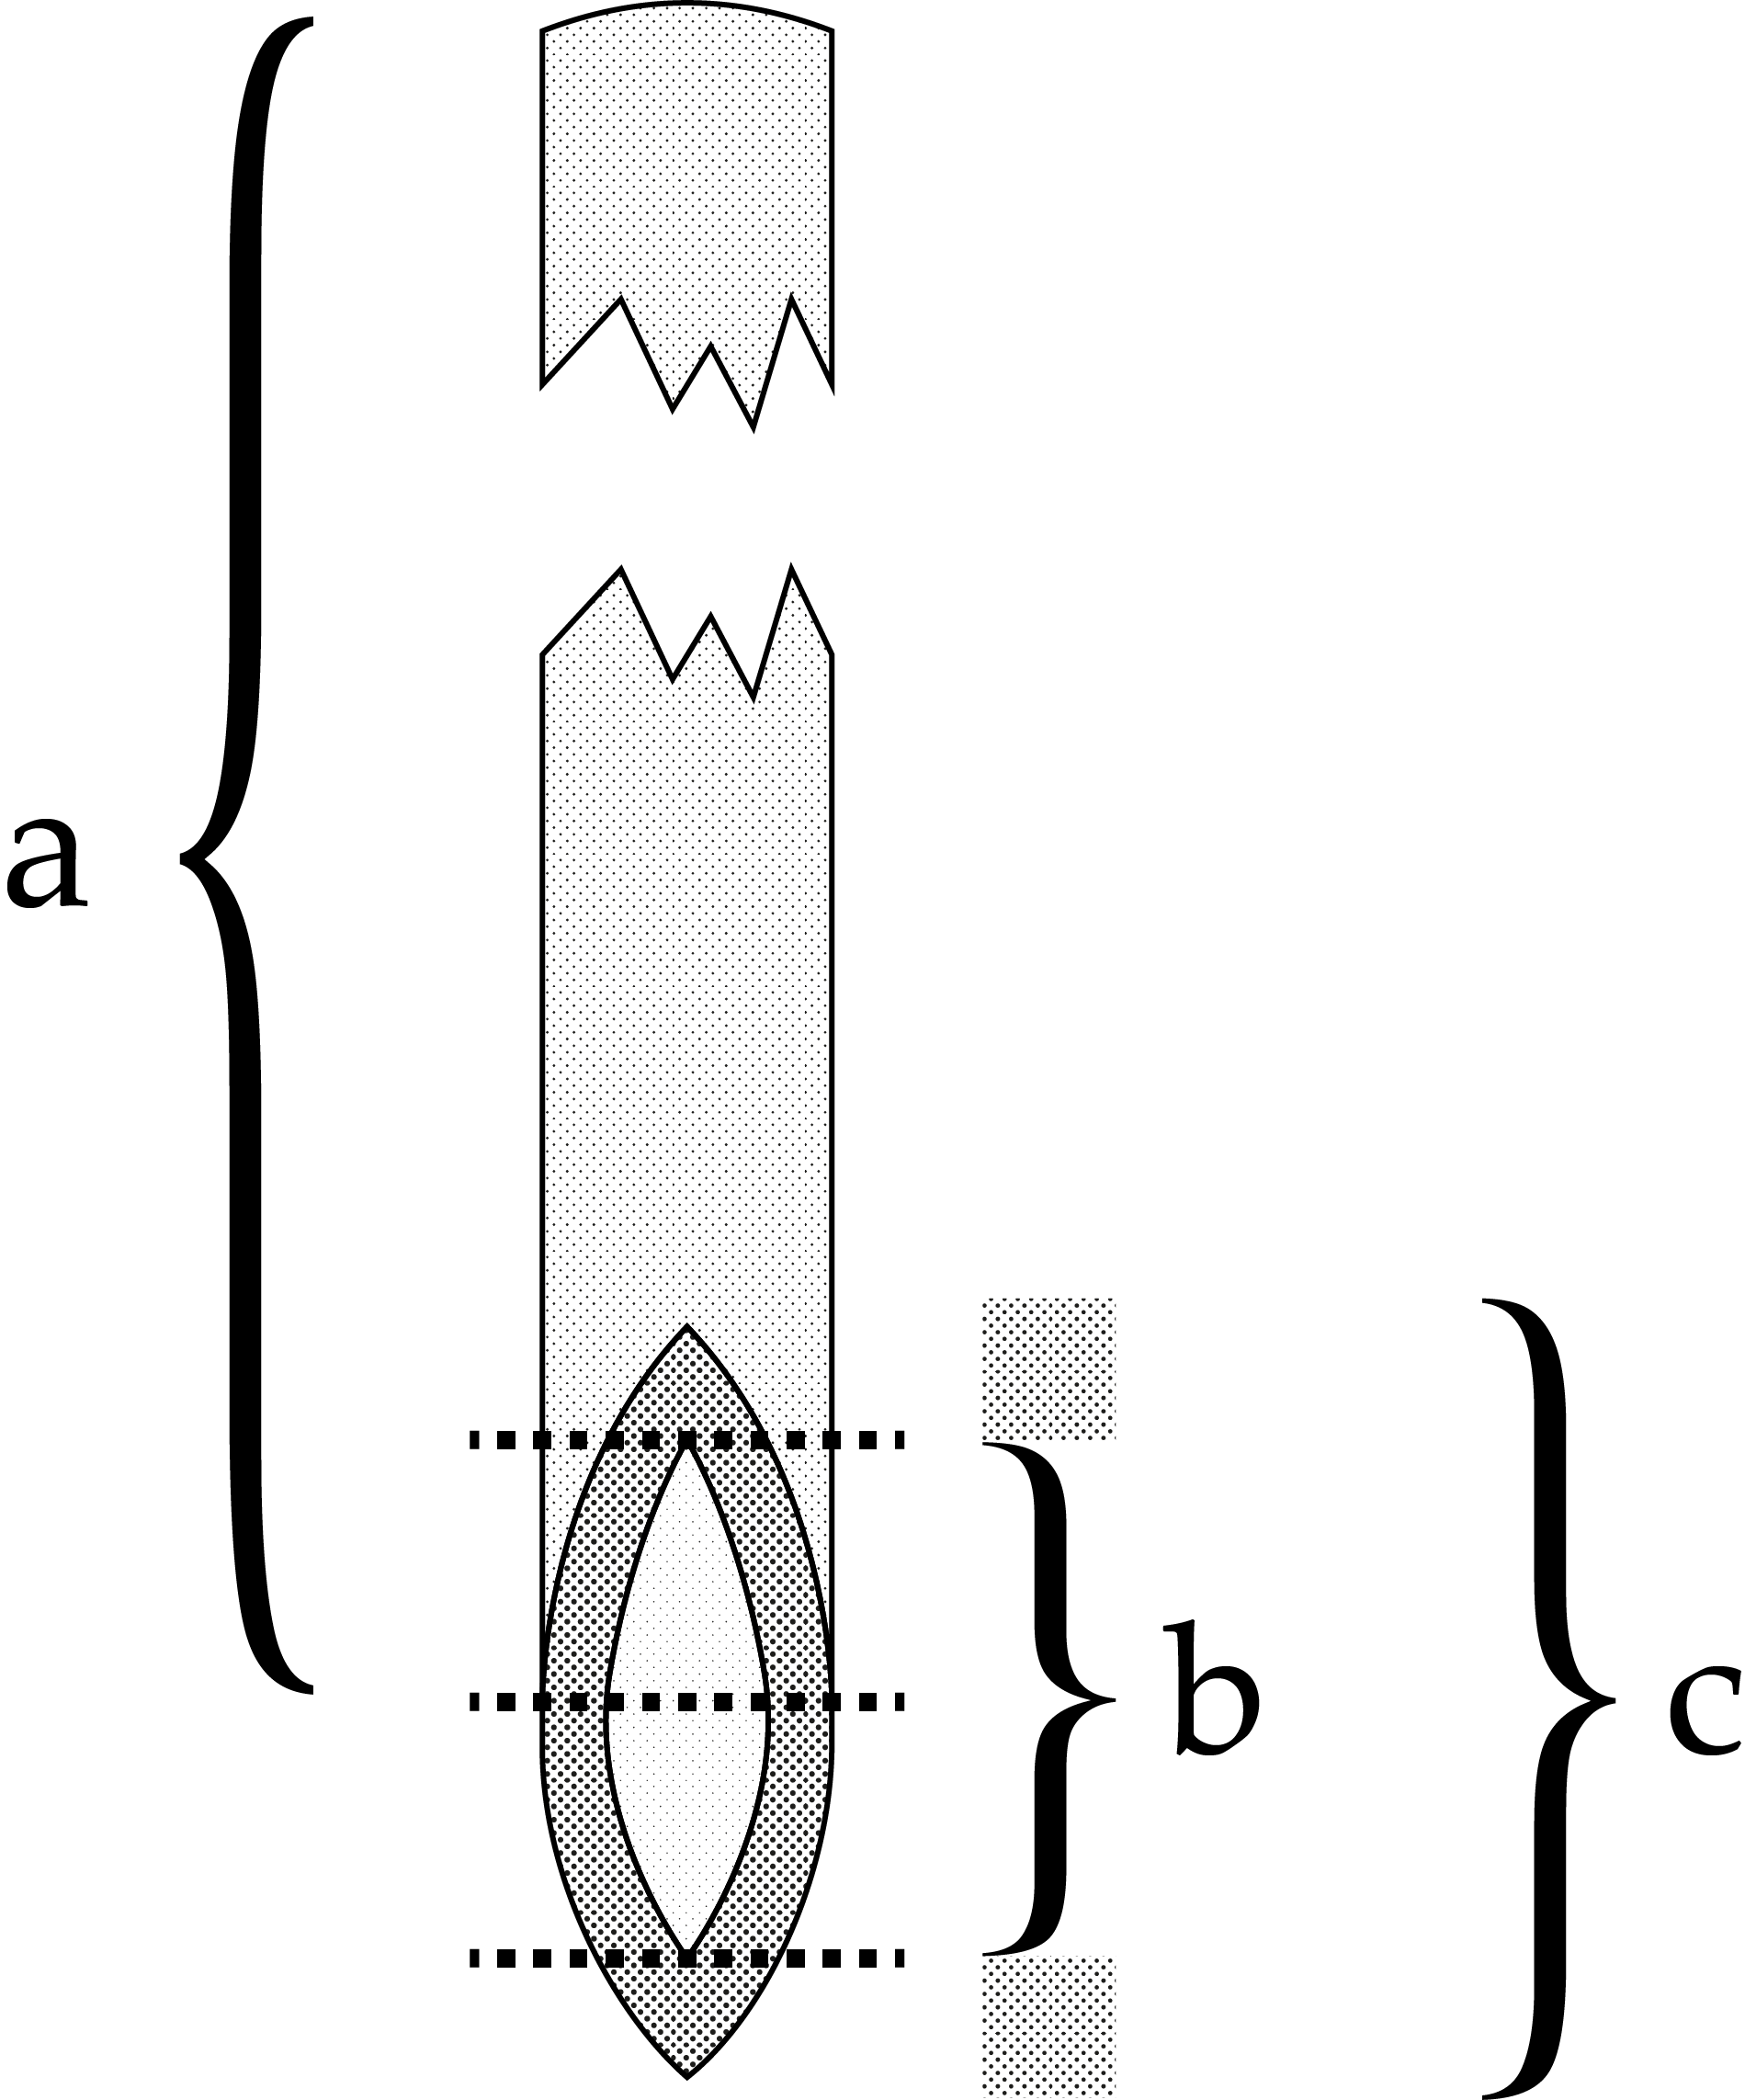
\includegraphics[width=110pt]{KapillareMasse.png}
\caption{Kapillare mit Länge (a), Unsicherheit durch Öffnung (b) und Unsicherheit durch Öffnung und Messfehler(c)}
\label{fig:length_eight_mouse}
\end{figure}
\noindent
Für alle fortgepflanzten Fehler wurden die Gleichungen aus Abschnitt 4.1 und 4.2 des ABW-Scriptes \cite{2} verwendet.
\section{Zusatzfragen}
\subsection{Fallschirmspringer}
Zur Vereinfachung nehmen wir an der Mensch sei ein Zylinder
mit Radius $r=0.25$ m, Höhe $h = 1,8$ m und einer Masse $m = 80
$ kg. Bestimmen wir mit
\begin{equation}
    r_K = \sqrt[3]{\frac{3}{4} \cdot r^2 \cdot h}
\end{equation}
den Radius $r_K$ einer Kugel, die im Wesentlichen das gleiche Volumen wie der Zylinder besitzt, lässt sich Gleichung 8 zur Bestimmung der Viskosität anwenden. Die Dichte des Fallschirmspringers erhalten wir mit
\begin{equation}
    \rho_M = \frac{3 \cdot m}{4\pi r_K^3} = 226,4   \frac{\textrm{kg}}{\textrm{m}^3}.
\end{equation}
Setzt man jetzt einen Literaturwert von $\rho_{Luft}= 1,2041 \frac{\textrm{kg}}{\textrm{m}^3}$ \cite{3} in Gleichung 8 ein, erhält man einen Wert von $\eta_{Luft} \approx 1,7$ Pa s, welcher ca. um einen Faktor $10^6$ größer als der Literaturwert $\eta_{Luft} = 18 \mu$ Pa s \cite{4} von trockener Luft bei $15 \degree $C ist. Höchstwahrscheinlich kommt diese enorme Abweichung von den extrem idealisierten Annahmen und der Tatsache, dass Gleichung 8 nur für laminare Strömungen gilt. Diese Strömungsart liegt jedoch nicht vor. Berechnet man nämlich die Reynoldszahl mit Gleichung 2 zu $R_e \approx 3,3 \cdot 10^7$, mit $L = 2 \cdot r_K$ und dem Literaturwert für $\eta_{Luft}$, so erkennt man, dass es sich beim freien Fall um eine turbulente Strömung handelt.

\subsection{Strömung in Nasenlöchern}
Wir nehmen an, dass man ungefähr 15 mal pro Minute je $0,5$ Liter Luft ein- und wieder ausatmet \cite{7}. Daraus folgt die Stromstärke $i = 25  $ cm$^3$/s. Der Radius eines Nasenlochs wird auf $r = 0,50$ cm geschätzt. Damit kommt man mit einem Nasenlochquerschnitt $A = 0,79$ cm$^2$ auf eine mittlere Strömungsgeschwindigkeit von $\nu= \frac{i}{A} = 3.2$ ms$^{-1}$. Unter Verwendung von $\rho_{Luft}= 1,29 \cdot 10^{-3}$ g/cm$^3$ \cite{1}, $L=d=2 \cdot r$ und dem Literaturwert $\eta_{Luft}$ aus der vorherigen Aufgabe wird die Reynoldszahl mit Gleichung 2 zu $R_e = 1147$ bestimmt. Wir nehmen außerdem an, dass der Luftstrom nur durch ein Nasenloch geht, da ein großer Teil der Menschen abwechselnd durch ein Nasenloch atmet \cite{5}. Eine Reynoldszahl von $1147$ ist schon im Bereich, in dem turbulente Strömung auftreten kann, jedoch ist dies aber eher unwahrscheinlich, da diese evolutionär schließlich nur für Luftströme entstanden sind und daher keine Einlaufstörungen verursachen sollte. Das Luftvolumen skaliert in diesem Beispiel linear mit der Reynoldszahl, so dass bei stärkerer Atmung, sagen wir, doppelt so schnell, sich demnach auch die Reynoldszahl verdoppelt. Mit $R_e \approx 2294$ ist man dann
im Grunde schon im Bereich turbulenter Strömung.
\section{Literaturverzeichnis}
\begin{thebibliography}{9}
\bibitem{1}
TUM Fakultät für Physik. \emph{Viskosität (VIS)}. 12.07.2022. \\
\textbf{URL:} \url{https://www.ph.tum.de/academics/org/labs/ap/ap1/VIS.pdf}
\bibitem{2}
TUM Fakultät für Physik. \emph{ABW-Skript} (12.07.2022). \\
\textbf{URL:} \url{https://www.ph.tum.de/academics/org/labs/ap/org/ABW.pdf}
\bibitem{3}
Wikipedia. \emph{Luftdichte} (12.07.2022). \\
\textbf{URL:} \url{https://de.wikipedia.org/wiki/Luftdichte}
\bibitem{4}
Wikibooks. \emph{Tabellensammlung Chemie/ Dynamische Viskosität gasförmiger Stoffe.} (12.07.2022). \\
\textbf{URL:}\url{https://de.wikibooks.org/wiki/Tabellensammlung_Chemie/_Dynamische_Viskosit%C3%A4t_gasf%C3%B6rmiger_Stoffe}
\bibitem{5}
Wikipedia. \emph{Nasenzyklus} (12.07.2022). \\
\textbf{URL:} \url{https://de.wikipedia.org/wiki/Nasenzyklus}
\bibitem{6}
Deutscher Kalibrierdienst. \emph{Nationaler Vergleich von Aräometerkalibrierungen} (12.07.2022). \\
\textbf{URL:} \url{https://oar.ptb.de/files/download/60c88a074c93901b9c005eab}
\bibitem{7}
Wikipedia. \emph{Atemminutenvolumen} (12.07.2022). \\
\textbf{URL:} \url{https://de.wikipedia.org/wiki/Atemminutenvolumen}
\bibitem{8}
Internetchemie.info. \emph{Wasser-Dichtetabelle} (17.07.2022). \\
\textbf{URL:} \url{https://www.internetchemie.info/chemie-lexikon/daten/w/wasser-dichtetabelle.php}
\bibitem{9}
H. Sigloh. \emph{Technische Fluidmechanik, Anhang, Tabelle 6-5}, Springer Verlag (17.07.2022). \\
\textbf{URL:} \url{https://link.springer.com/content/pdf/bbm$\%$3A978-3-540-44635-4%2F1}
\end{thebibliography}
\section{Anhang}
\subsection{Laborbuch}
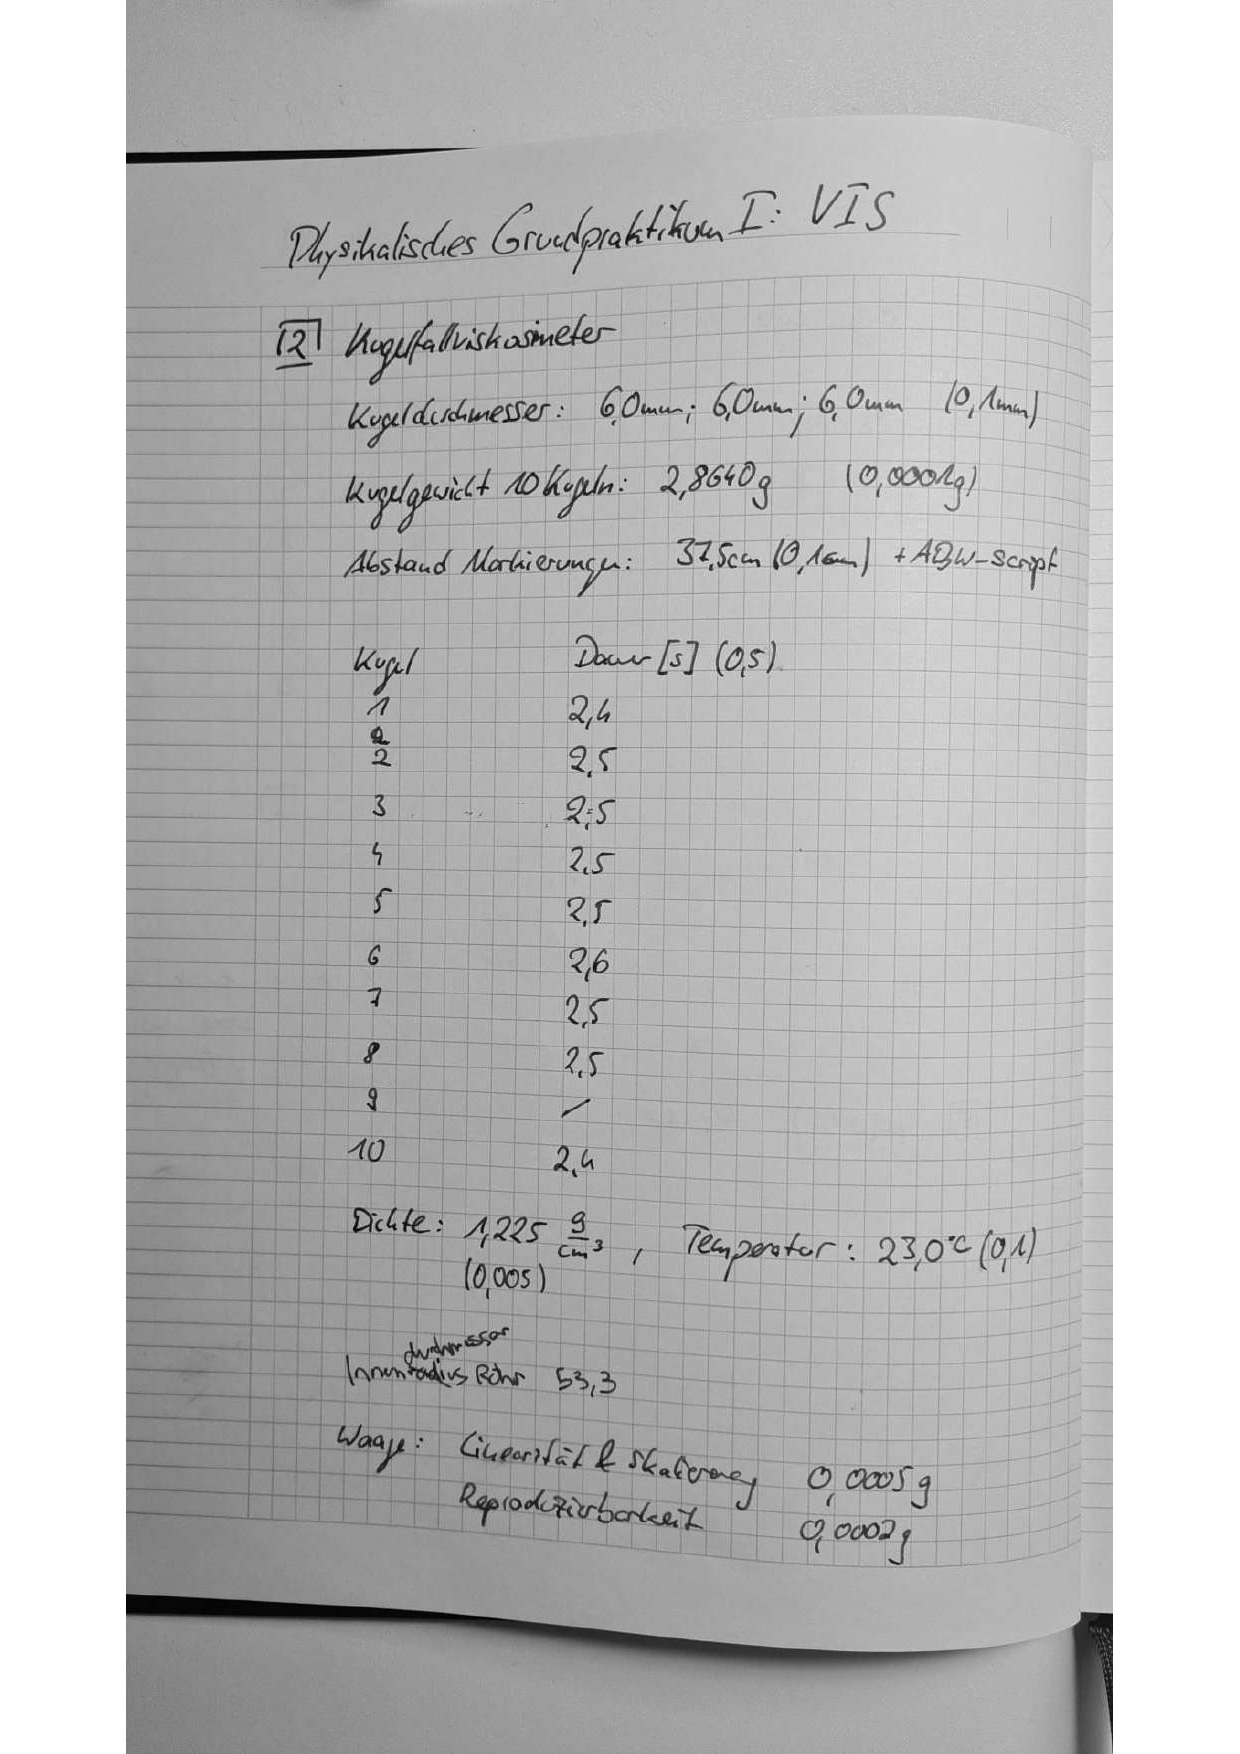
\includepdf[pages=-]{Protokoll.pdf}
\end{document}

